\documentclass[11pt]{article}

\usepackage[a4paper,margin=1in]{geometry}
\usepackage[T1]{fontenc}
\usepackage[utf8]{inputenc}
\usepackage{lmodern}
\usepackage{microtype}
\usepackage{amsmath}
\usepackage{amssymb}
\usepackage{booktabs}
\usepackage{longtable}
\usepackage{array}
\usepackage{xcolor}
\usepackage{hyperref}
\usepackage{enumitem}
\usepackage{tikz}
\usetikzlibrary{arrows.meta,positioning,shapes.geometric,fit,backgrounds}

\hypersetup{
  colorlinks=true,
  linkcolor=blue!60!black,
  urlcolor=blue!60!black
}

\setlist[itemize]{leftmargin=1.5em}
\setlist[enumerate]{leftmargin=1.6em}

\title{EEG-to-Word Decoding Project: Consolidated Findings, Current Architecture, and Next Research Directions}
\author{Project Documentation}
\date{April 2026}

\begin{document}
\maketitle

\begin{abstract}
This document consolidates the project findings obtained while trying to reproduce and exceed BELT-style EEG-to-word classification performance on ZuCo. It summarizes the baseline BELT-style setup, the enhanced training attempts, the raw fixation-level EEG+eye-tracking pipeline, the grouped raw word-level pipeline, and the current hybrid processed+raw architecture. It also records the reasons behind each design choice, the main failure modes observed so far, and the highest-priority research directions for the next phase. The goal is not only to preserve what was tried, but also to prevent future work from repeating low-yield experiments and to make the next implementation stage more deliberate and research-grounded.
\end{abstract}

\tableofcontents
\newpage

\section{Project Goal}

The main goal of this project is to perform \textbf{EEG-to-word classification} over a \textbf{500-word vocabulary} using ZuCo reading data, while trying to:
\begin{itemize}
    \item reproduce BELT-style performance faithfully,
    \item understand why the current repository saturates below the BELT paper's reported score,
    \item and ultimately build a stronger architecture that can surpass the best processed-feature baseline.
\end{itemize}

The practical metric that has served as the main anchor throughout this work is:
\begin{itemize}
    \item \textbf{Top-10 accuracy}
\end{itemize}

This was chosen because:
\begin{itemize}
    \item it is the metric prominently discussed in BELT-style comparisons,
    \item Top-1 accuracy showed a collapsed prediction pattern in several runs,
    \item and Top-10 retained useful discriminative signal even when Top-1 did not.
\end{itemize}

\section{What BELT Contributes Conceptually}

BELT, in its core form, is not simply ``processed EEG plus classifier.'' Its conceptual ingredients are:
\begin{enumerate}
    \item A \textbf{strong encoder} over processed EEG features.
    \item A \textbf{discrete bottleneck} through vector quantization (VQ).
    \item \textbf{language-side supervision} through an EEG-language alignment objective.
\end{enumerate}

In this repository, that family is represented by:
\begin{itemize}
    \item processed frequency-band EEG summaries of size \(840 = 105 \times 8\),
    \item a D-Conformer encoder,
    \item an optional vector quantizer,
    \item an MLP classifier,
    \item and, in some variants, a BART-based contrastive objective.
\end{itemize}

The original motivation for moving beyond BELT was that the repository repeatedly saturated near the \(\sim 29.5\%\) Top-10 band rather than crossing the reported \(31.04\%\) region.

\section{Chronology of the Main Findings}

\subsection{Processed BELT-Style Replica}

The processed-feature BELT-style path established the strongest initial anchor:
\begin{itemize}
    \item Best observed processed baseline band: about \textbf{29.4--29.55\% Top-10}
    \item Stronger training tricks, richer fused summary inputs, class-balanced CE, and weighted sampling did \textbf{not} create a meaningful jump beyond that band.
\end{itemize}

Important conclusions from this stage:
\begin{itemize}
    \item The repository had a \textbf{real, stable processed-feature baseline}.
    \item The missing improvement was \textbf{not} explained by simple optimizer, sampler, or CE weighting changes.
    \item The contrastive branch, in its current implementation, was at best weakly helpful and often ineffective.
\end{itemize}

\subsection{Processed Path Diagnostics}

The most important processed-path findings were:
\begin{itemize}
    \item Weighted sampling hurt training instead of helping.
    \item Class-balanced CE also degraded behavior.
    \item The improved/enhanced stack with many tricks still stayed in essentially the same Top-10 band.
    \item Top-1 behavior frequently looked frequency-collapsed, often tracking dominant words such as \texttt{the}.
\end{itemize}

This strongly suggested that the main issue was \textbf{not} ``lack of training tricks.'' It pointed instead toward a more structural bottleneck:
\begin{itemize}
    \item representation quality,
    \item context modeling,
    \item or mismatch between current supervision and the actual decoding problem.
\end{itemize}

\subsection{Raw Fixation-Level Pipeline}

To move beyond handcrafted summaries, a new raw pipeline was built using:
\begin{itemize}
    \item raw fixation-level EEG windows,
    \item raw eye-tracking sequences,
    \item fixation statistics such as \texttt{FFD}, \texttt{GD}, \texttt{TRT}, and related gaze metrics.
\end{itemize}

This was a major preprocessing step because it preserved temporal structure that BELT-style band summaries remove.

However, the \textbf{first raw fixation-level model} underperformed:
\begin{itemize}
    \item it learned,
    \item but plateaued in the low-\(23\%\) Top-10 region on dev,
    \item far below the processed baseline.
\end{itemize}

This was a critical finding:
\begin{itemize}
    \item raw signal contains more information,
    \item but it also contains much more nuisance variation and is harder to learn from.
\end{itemize}

\subsection{Grouped Raw Word-Level Pipeline}

The first major raw-data improvement was to \textbf{group fixations by word} rather than predict from isolated fixations. This changed the problem from:
\begin{itemize}
    \item ``predict word from one noisy fixation''
\end{itemize}
to:
\begin{itemize}
    \item ``predict word from the grouped raw temporal evidence associated with that word.''
\end{itemize}

This produced a large improvement:
\begin{itemize}
    \item raw fixation-level best band: around \textbf{23.6\%}
    \item grouped + normalized raw word-level best band: around \textbf{28.24\%}
\end{itemize}

This was one of the most important results in the project.

\paragraph{Interpretation.}
It proved that \textbf{preprocessing mattered a lot}, especially:
\begin{itemize}
    \item grouping fixations correctly,
    \item preserving temporal information,
    \item and normalizing raw sequences.
\end{itemize}

At the same time, it also showed that preprocessing alone did \textbf{not} close the full gap to the processed baseline.

\subsection{Current Hybrid Processed+Raw Pipeline}

A hybrid model was then built to combine:
\begin{itemize}
    \item a BELT-style processed summary branch,
    \item a grouped raw EEG+ET branch,
    \item and a gated fusion module.
\end{itemize}

The intuition was straightforward:
\begin{itemize}
    \item processed features are low-noise and already strong,
    \item raw features preserve temporal detail,
    \item so combining both should outperform either branch alone.
\end{itemize}

What actually happened:
\begin{itemize}
    \item the hybrid model learned stably,
    \item but it plateaued near \textbf{28.2\% Top-10},
    \item still below the strongest processed baseline.
\end{itemize}

This means:
\begin{itemize}
    \item simple fusion is not enough,
    \item raw signal is useful,
    \item but the way the current hybrid organizes and supervises representation is still too weak.
\end{itemize}

\section{Summary Table of Main Experimental Regimes}

\begin{longtable}{p{3.2cm}p{4.8cm}p{3.0cm}p{3.6cm}}
\toprule
\textbf{Regime} & \textbf{Core Input / Idea} & \textbf{Observed Best Band} & \textbf{Main Conclusion} \\
\midrule
\endfirsthead
\toprule
\textbf{Regime} & \textbf{Core Input / Idea} & \textbf{Observed Best Band} & \textbf{Main Conclusion} \\
\midrule
\endhead
Processed BELT-style baseline & \(840\)-dim processed EEG summary features, D-Conformer family, CE-focused baseline anchor & \(\sim 29.4\) to \(\sim 29.55\%\) Top-10 & Strongest stable anchor so far \\
Enhanced processed training & Same processed family with additional tricks, regularization, alternate losses & Still \(\sim 29\%\) band & Training tricks did not solve the bottleneck \\
Raw fixation-level & Raw EEG+ET per fixation, temporal modeling from isolated fixation windows & \(\sim 23.6\%\) & Raw-only at fixation granularity is too noisy \\
Grouped raw word-level & Grouped raw fixations for each word + normalization + temporal patching & \(\sim 28.24\%\) & Big preprocessing win, but still below processed baseline \\
Hybrid processed+raw (current) & Processed summary branch + grouped raw EEG+ET branch + gated fusion, CE only & \(\sim 28.2\%\) & Fusion alone is not enough; stronger supervision is needed \\
\bottomrule
\end{longtable}

\section{Why Each Major Change Was Tried}

\subsection{Why Move Beyond Processed EEG Summaries?}

The processed BELT-style path already performed reasonably well, but it had clear limitations:
\begin{itemize}
    \item it compresses away within-fixation temporal dynamics,
    \item it uses band-level summaries rather than raw spatiotemporal signal,
    \item and it risks making the sequence model underused.
\end{itemize}

So the raw path was introduced because the current bottleneck could plausibly be due to:
\begin{itemize}
    \item over-compression of the signal,
    \item information loss during preprocessing,
    \item or inability of processed features to retain reading-specific timing structure.
\end{itemize}

\subsection{Why Group Fixations by Word?}

Predicting from one fixation at a time created a harder problem than the actual reading behavior suggests. A word can be:
\begin{itemize}
    \item fixated more than once,
    \item revisited,
    \item associated with multiple temporal response fragments.
\end{itemize}

Grouping fixations by word was intended to:
\begin{itemize}
    \item reduce label noise,
    \item better match the actual prediction target,
    \item and aggregate useful evidence scattered across fixations.
\end{itemize}

The strong improvement from grouped raw words confirmed that this was the right move.

\subsection{Why Add Eye-Tracking?}

This was motivated by both intuition and reading-task structure:
\begin{itemize}
    \item eye movements directly reflect the act of reading,
    \item gaze behavior and EEG are temporally linked during fixation,
    \item and multimodal fusion is often better than either modality alone in reading-related tasks.
\end{itemize}

Even if the eye-tracking branch is not yet sufficient to break the baseline, it is still a valuable signal source and should likely remain in future models.

\subsection{Why Build a Hybrid Model?}

The hybrid idea came from the observation that:
\begin{itemize}
    \item processed features are low-noise and already strong,
    \item raw features provide detail that processed features discard,
    \item and a good fusion model should, in principle, get the best of both worlds.
\end{itemize}

The fact that the current hybrid still plateaued implies not that the idea is wrong, but that:
\begin{itemize}
    \item the current form of fusion is too weak,
    \item the processed branch is too shallow compared with BELT's actual encoder,
    \item and the supervision objective is still insufficient.
\end{itemize}

\section{Current Architecture}

\subsection{Current Hybrid Pipeline at a High Level}

\begin{center}
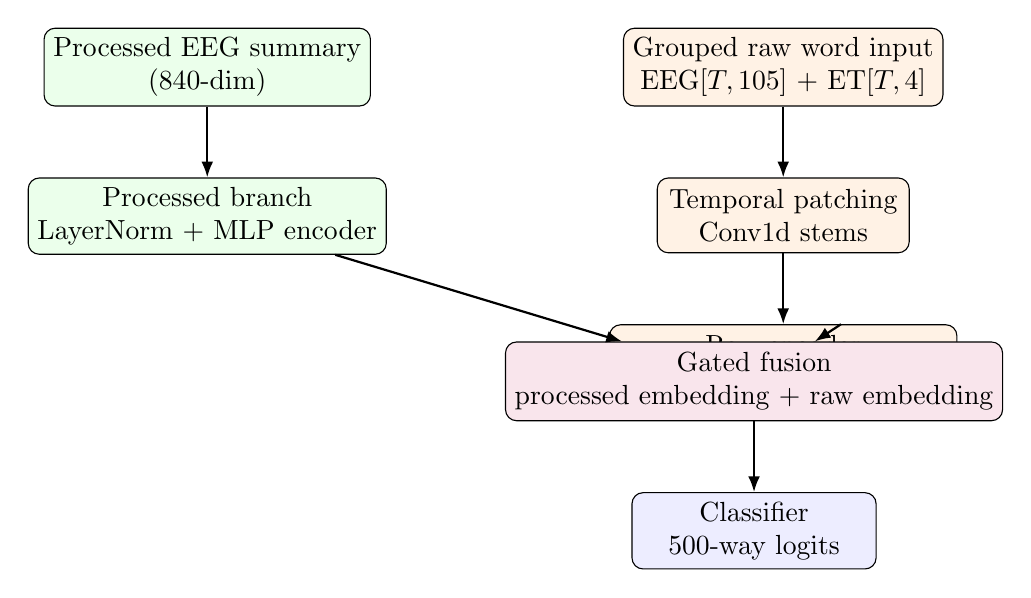
\begin{tikzpicture}[
    node distance=0.9cm and 0.8cm,
    block/.style={draw, rounded corners, align=center, minimum width=3.1cm, minimum height=0.95cm, fill=blue!7},
    proc/.style={draw, rounded corners, align=center, minimum width=3.1cm, minimum height=0.95cm, fill=green!8},
    raw/.style={draw, rounded corners, align=center, minimum width=3.2cm, minimum height=0.95cm, fill=orange!10},
    fuse/.style={draw, rounded corners, align=center, minimum width=3.6cm, minimum height=1.0cm, fill=purple!10},
    arr/.style={-{Latex[length=2mm]}, thick}
]
\node[proc] (procin) {Processed EEG summary\\(\(840\)-dim)};
\node[proc, below=of procin] (procenc) {Processed branch\\LayerNorm + MLP encoder};

\node[raw, right=3.2cm of procin] (rawin) {Grouped raw word input\\EEG[\(T,105\)] + ET[\(T,4\)]};
\node[raw, below=of rawin] (rawstem) {Temporal patching\\Conv1d stems};
\node[raw, below=of rawstem] (rawenc) {Raw encoder\\Transformer + aux metrics};

\node[fuse, below right=1.1cm and 1.5cm of procenc] (fusion) {Gated fusion\\processed embedding + raw embedding};
\node[block, below=of fusion] (clf) {Classifier\\500-way logits};

\draw[arr] (procin) -- (procenc);
\draw[arr] (rawin) -- (rawstem);
\draw[arr] (rawstem) -- (rawenc);
\draw[arr] (procenc) -- (fusion);
\draw[arr] (rawenc) -- (fusion);
\draw[arr] (fusion) -- (clf);
\end{tikzpicture}
\end{center}

\subsection{Current Hybrid Implementation Details}

The current hybrid architecture contains:
\begin{itemize}
    \item a \textbf{processed branch} that maps a processed EEG vector into a model embedding,
    \item a \textbf{raw EEG branch} with temporal patching,
    \item a \textbf{raw eye-tracking branch},
    \item \textbf{gated raw fusion} between EEG and eye-tracking,
    \item an auxiliary \textbf{metrics projection} for hand-crafted fixation features,
    \item a \textbf{TransformerEncoder} over temporally downsampled raw sequences,
    \item a \textbf{gated hybrid fusion} between processed and raw embeddings,
    \item and a final classifier head.
\end{itemize}

In code terms, this is represented by the model in:
\begin{itemize}
    \item \texttt{models/hybrid\_processed\_raw.py}
\end{itemize}

with configuration in:
\begin{itemize}
    \item \texttt{config/hybrid\_processed\_raw\_mixed.yaml}
\end{itemize}

\subsection{Current Hybrid Configuration Snapshot}

The main current settings are:
\begin{itemize}
    \item processed dimension: \(840\)
    \item EEG dimension: \(105\)
    \item ET dimension: \(4\)
    \item model dimension: \(192\)
    \item attention heads: \(6\)
    \item transformer layers: \(3\)
    \item patch stride: \(4\)
    \item loss: plain cross-entropy only
\end{itemize}

\subsection{Current Architecture Versus BELT}

At the benchmark level, the project is still close to BELT because it keeps:
\begin{itemize}
    \item the 500-word classification task,
    \item Top-\(k\) accuracy evaluation,
    \item and one processed summary branch.
\end{itemize}

At the model level, however, the current hybrid is now far from BELT:
\begin{itemize}
    \item the processed branch is no longer the full BELT D-Conformer branch,
    \item there is no active VQ in the current hybrid,
    \item there is no active language alignment loss in the current hybrid,
    \item and the raw multimodal branch is entirely new.
\end{itemize}

So the current model should be thought of as:
\begin{quote}
``a BELT-derived benchmark with a new hybrid architecture,''
\end{quote}
not as a faithful BELT implementation.

\section{BELT Versus Current Hybrid: The Real Gap}

\subsection{BELT-Style Pipeline}

\begin{center}
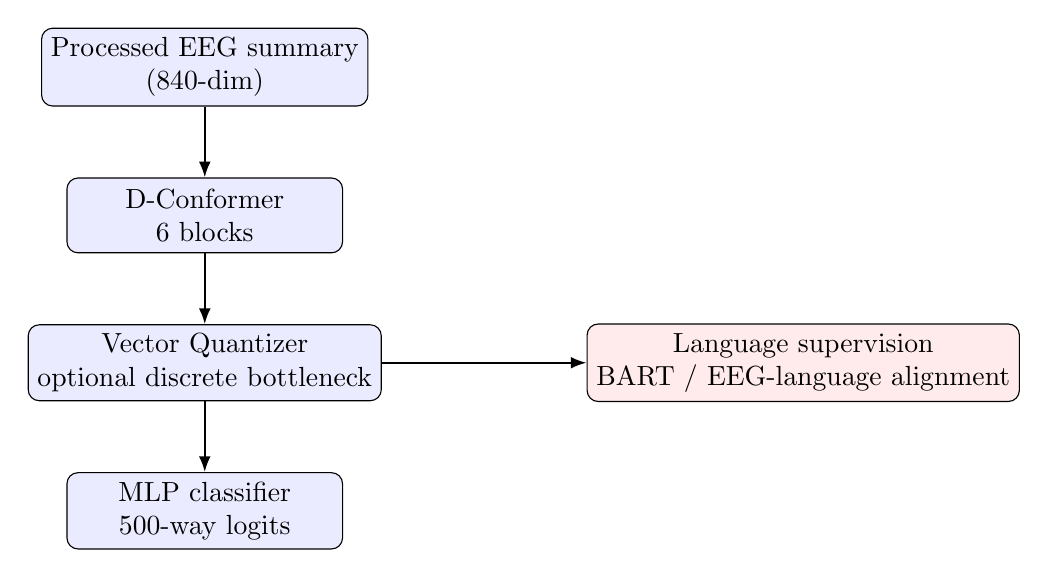
\begin{tikzpicture}[
    node distance=0.9cm and 0.8cm,
    block/.style={draw, rounded corners, align=center, minimum width=3.5cm, minimum height=0.95cm, fill=blue!8},
    loss/.style={draw, rounded corners, align=center, minimum width=3.3cm, minimum height=0.95cm, fill=red!8},
    arr/.style={-{Latex[length=2mm]}, thick}
]
\node[block] (x) {Processed EEG summary\\(\(840\)-dim)};
\node[block, below=of x] (enc) {D-Conformer\\6 blocks};
\node[block, below=of enc] (vq) {Vector Quantizer\\optional discrete bottleneck};
\node[block, below=of vq] (clf) {MLP classifier\\500-way logits};
\node[loss, right=2.6cm of vq] (lang) {Language supervision\\BART / EEG-language alignment};

\draw[arr] (x) -- (enc);
\draw[arr] (enc) -- (vq);
\draw[arr] (vq) -- (clf);
\draw[arr] (vq) -- (lang);
\end{tikzpicture}
\end{center}

\subsection{What the Current Hybrid Removed}

Compared to full BELT-like behavior, the current hybrid removed or weakened:
\begin{itemize}
    \item the \textbf{full processed D-Conformer branch},
    \item the \textbf{discrete bottleneck},
    \item and the \textbf{language-side alignment objective}.
\end{itemize}

These are exactly the three components most tied to BELT's core identity.

\subsection{Why This Matters}

The current hybrid already showed that:
\begin{itemize}
    \item extra signal alone is not enough,
    \item and simple CE-only fusion does not create the missing gain.
\end{itemize}

This strongly suggests that the next useful model should not be:
\begin{itemize}
    \item raw-only,
    \item or CE-only hybrid,
    \item or another training-trick-heavy processed model.
\end{itemize}

Instead, the most grounded next design is:
\begin{quote}
\textbf{BELT core processed encoder + grouped raw branch + stronger language-aware supervision}
\end{quote}

\section{What the Results Actually Tell Us}

\subsection{What We Can Say with Confidence}

\begin{enumerate}
    \item The repository already has a strong processed baseline near \(\sim 29.5\%\) Top-10.
    \item Raw fixation-level modeling is too noisy when done at isolated-fixation granularity.
    \item Grouping fixations to word level is a major improvement and should be retained.
    \item Raw temporal information is useful, but not sufficient by itself.
    \item Simple processed+raw fusion with CE is also not sufficient by itself.
    \item The remaining gap is now more likely in \textbf{representation organization, fusion strategy, and supervision objective} than in basic preprocessing mistakes.
\end{enumerate}

\subsection{What We Should Avoid Concluding Too Strongly}

The following would be overclaims:
\begin{itemize}
    \item that raw EEG is useless,
    \item that VQ never helps,
    \item that contrastive or alignment losses are pointless,
    \item or that more data can never help.
\end{itemize}

The correct conclusion is narrower:
\begin{itemize}
    \item the \textbf{current forms} of raw-only modeling, CE-only fusion, and existing contrastive usage have not produced the breakthrough yet.
\end{itemize}

\section{Real Problems Identified So Far}

\subsection{Problem 1: Weak Supervision Relative to the Difficulty of the Input}

Raw EEG+ET is a much harder representation learning problem than processed summary decoding. Yet the current hybrid still uses:
\begin{itemize}
    \item plain CE,
    \item no contextual semantic target,
    \item and no language-aware fusion mechanism.
\end{itemize}

This likely makes the model under-supervised for the complexity of the input.

\subsection{Problem 2: Current Hybrid Is Not Truly ``BELT + Ours''}

The current hybrid uses a processed branch, but not the actual BELT processed backbone. This matters because:
\begin{itemize}
    \item BELT's strongest prior is not just the processed features,
    \item it is the encoder structure plus the language-side supervision.
\end{itemize}

\subsection{Problem 3: Context Is Still Underused}

Even after moving to grouped words, the model is still largely trying to decode a word from the evidence tied only to that word. It is not yet strongly using:
\begin{itemize}
    \item neighboring words,
    \item sentence structure,
    \item contextual token identity,
    \item or reading-order context.
\end{itemize}

\subsection{Problem 4: Join Coverage Is Imperfect}

The hybrid cache builder revealed non-trivial mismatch counts, especially for some TSR-2.0 shards. This means:
\begin{itemize}
    \item the joined hybrid training set is smaller than the full raw set,
    \item some raw examples could not be paired with processed features,
    \item and tokenization/index alignment still contains edge cases.
\end{itemize}

\subsection{Problem 5: SR Is Missing in the Mixed Hybrid Setting}

The current mixed hybrid excludes SR because SR does not extend naturally into the cross-version 2.0 task overlap used for the raw pipeline. This was an engineering decision, not a proven accuracy win. Therefore:
\begin{itemize}
    \item there is no strong evidence yet that excluding SR helps the score,
    \item and it remains possible that a v1-only hybrid with SR could score better.
\end{itemize}

\section{What Is Most Likely to Produce Real Progress}

Based on all observed results so far, the highest-probability next direction is:

\begin{enumerate}
    \item Replace the current processed MLP branch with the actual \textbf{D-Conformer} processed branch.
    \item Keep the grouped raw EEG+ET branch.
    \item Fuse the two branches with a stronger fusion design.
    \item Add \textbf{contextual semantic alignment} instead of isolated-word contrastive matching.
\end{enumerate}

\subsection{Recommended Next Architecture}

\begin{center}
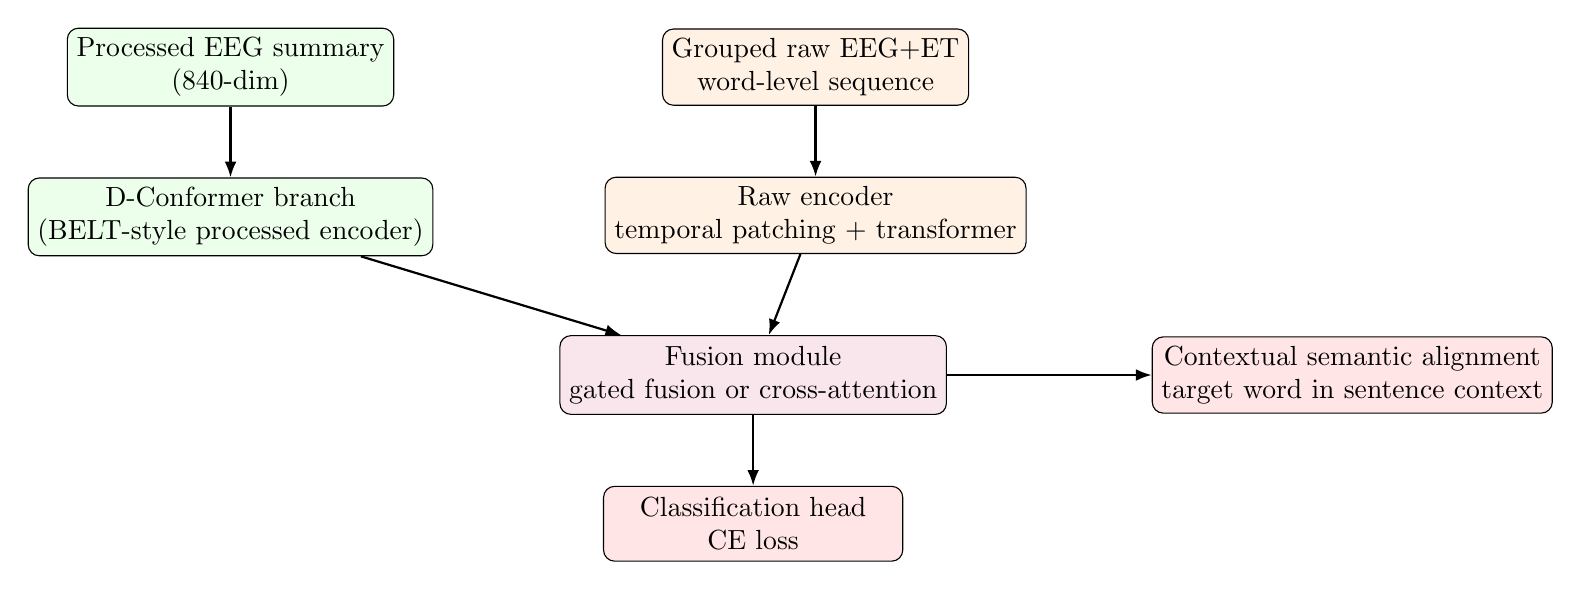
\begin{tikzpicture}[
    node distance=0.9cm and 0.8cm,
    proc/.style={draw, rounded corners, align=center, minimum width=3.1cm, minimum height=0.95cm, fill=green!8},
    raw/.style={draw, rounded corners, align=center, minimum width=3.3cm, minimum height=0.95cm, fill=orange!10},
    fuse/.style={draw, rounded corners, align=center, minimum width=3.8cm, minimum height=1.0cm, fill=purple!10},
    loss/.style={draw, rounded corners, align=center, minimum width=3.8cm, minimum height=0.95cm, fill=red!10},
    arr/.style={-{Latex[length=2mm]}, thick}
]
\node[proc] (p1) {Processed EEG summary\\(\(840\)-dim)};
\node[proc, below=of p1] (p2) {D-Conformer branch\\(BELT-style processed encoder)};

\node[raw, right=3.4cm of p1] (r1) {Grouped raw EEG+ET\\word-level sequence};
\node[raw, below=of r1] (r2) {Raw encoder\\temporal patching + transformer};

\node[fuse, below right=1.0cm and 1.6cm of p2] (f) {Fusion module\\gated fusion or cross-attention};
\node[loss, below=of f] (ce) {Classification head\\CE loss};
\node[loss, right=2.6cm of f] (ctx) {Contextual semantic alignment\\target word in sentence context};

\draw[arr] (p1) -- (p2);
\draw[arr] (r1) -- (r2);
\draw[arr] (p2) -- (f);
\draw[arr] (r2) -- (f);
\draw[arr] (f) -- (ce);
\draw[arr] (f) -- (ctx);
\end{tikzpicture}
\end{center}

\subsection{Why This Is the Best Next Step}

This design combines:
\begin{itemize}
    \item BELT's strongest processed representation prior,
    \item the most useful raw contribution discovered so far,
    \item and the supervision component that is currently missing.
\end{itemize}

In other words, it is the first proposal that genuinely tests:
\begin{quote}
``BELT core strengths + our strongest new signal path + stronger language-aware supervision.''
\end{quote}

\section{Why Not Simply Add VQ, Contrastive, or Focal Loss Immediately?}

\subsection{VQ}

VQ may still be useful, but not as the first next step. The project already saw:
\begin{itemize}
    \item only modest or inconsistent gains from current VQ usage,
    \item and no evidence that simply restoring a classifier-side VQ bottleneck would solve the main gap.
\end{itemize}

If VQ returns later, it should likely return in a more modern role:
\begin{itemize}
    \item residual vector quantization,
    \item tokenizer-style latent discretization,
    \item or masked pretraining.
\end{itemize}

\subsection{Contrastive Loss}

The current repo's contrastive path is too weak in its current form because it is closer to isolated-word supervision than to contextual semantic alignment. The next language loss should therefore be:
\begin{itemize}
    \item contextual,
    \item sentence-aware,
    \item and attached to the fused representation.
\end{itemize}

\subsection{Focal Loss}

Focal loss may still help later, especially if class skew remains a problem. However, the experiments already showed that:
\begin{itemize}
    \item weighted sampling hurt,
    \item class-balanced CE hurt,
    \item and representation quality appears to be a larger bottleneck than loss reweighting.
\end{itemize}

So focal loss is a lower-priority tool than fixing representation and supervision.

\section{Current Research Directions Worth Studying}

The next phase should not be guided by vague browsing. It should focus on specific research themes that match the current bottlenecks.

\subsection{Theme 1: Contextual EEG-Language Alignment}

\textbf{Why it matters:} the current supervision is too weak and too word-local.

\textbf{What to look for:}
\begin{itemize}
    \item contextual token alignment
    \item EEG-language alignment
    \item EEG semantic retrieval
    \item sentence-conditioned EEG decoding
    \item LLM-guided EEG decoding
    \item contextual word embeddings for EEG
\end{itemize}

\textbf{Implementation idea:}
\begin{itemize}
    \item build a sentence encoder for the word's sentence,
    \item extract the target token's contextual embedding,
    \item align the fused EEG representation to that embedding.
\end{itemize}

\subsection{Theme 2: Better Multimodal Fusion}

\textbf{Why it matters:} the current gated fusion is helpful but still weak.

\textbf{What to look for:}
\begin{itemize}
    \item cross-attention fusion EEG eye-tracking
    \item multimodal reading decoding
    \item hierarchical fusion EEG ET
    \item token-level multimodal fusion
\end{itemize}

\textbf{Implementation idea:}
\begin{itemize}
    \item replace simple late gating with cross-attention or dual-stream co-attention.
\end{itemize}

\subsection{Theme 3: Hierarchical Reading Models}

\textbf{Why it matters:} grouped word-level modeling was a big improvement, which suggests that hierarchical structure matters.

\textbf{What to look for:}
\begin{itemize}
    \item fixation-to-word modeling
    \item word-to-sentence EEG models
    \item hierarchical EEG transformers
    \item reading order modeling
    \item scanpath-aware decoding
\end{itemize}

\textbf{Implementation idea:}
\begin{itemize}
    \item first encode fixations within a word,
    \item then encode neighboring words within sentence order.
\end{itemize}

\subsection{Theme 4: Foundation EEG Encoders and State-Space Models}

\textbf{Why it matters:} raw EEG is long, noisy, and expensive for ordinary transformers.

\textbf{What to look for:}
\begin{itemize}
    \item EEG foundation model
    \item pretrained EEG encoder
    \item LaBraM
    \item EEG-FM benchmark
    \item EEG Mamba
    \item state-space model EEG
    \item patch EEG transformer
\end{itemize}

\textbf{Implementation idea:}
\begin{itemize}
    \item initialize the raw branch from a pretrained EEG encoder,
    \item or replace the raw transformer with a better long-sequence backbone.
\end{itemize}

\subsection{Theme 5: Modern Quantization / Tokenization}

\textbf{Why it matters:} VQ is not dead; the current usage may simply be the wrong form.

\textbf{What to look for:}
\begin{itemize}
    \item residual vector quantization EEG
    \item EEG tokenization
    \item neural tokenizer EEG
    \item masked latent EEG modeling
    \item discrete EEG representation learning
\end{itemize}

\textbf{Implementation idea:}
\begin{itemize}
    \item use VQ/RVQ for pretraining or tokenization,
    \item not just as a direct bottleneck inside a classifier stack.
\end{itemize}

\subsection{Theme 6: Data and Preprocessing Refinements}

\textbf{Why it still matters:} preprocessing is no longer the only issue, but it is still not fully solved.

\textbf{What to look for:}
\begin{itemize}
    \item subject normalization EEG decoding
    \item session normalization EEG
    \item blink artifact reading EEG
    \item fixation onset windowing
    \item robust scaling EEG
    \item multimodal preprocessing EEG eye-tracking
\end{itemize}

\textbf{Implementation idea:}
\begin{itemize}
    \item improve per-subject and per-session normalization,
    \item re-check join coverage and TSR-2.0 alignment,
    \item test more principled temporal cropping around fixation events.
\end{itemize}

\section{Suggested Search Keywords for the Next Research Cycle}

To keep the next phase focused, the following keyword sets are recommended.

\subsection{Core Semantic Alignment Keywords}

\begin{itemize}
    \item EEG language alignment
    \item contextual semantic alignment EEG
    \item EEG text retrieval
    \item sentence-conditioned EEG decoding
    \item contextual embedding EEG reading
    \item reading EEG semantic decoding
\end{itemize}

\subsection{Multimodal Reading Keywords}

\begin{itemize}
    \item EEG eye-tracking fusion reading
    \item multimodal reading decoding EEG ET
    \item gaze EEG word prediction
    \item reading comprehension EEG eye-tracking
\end{itemize}

\subsection{Sequence Modeling Keywords}

\begin{itemize}
    \item EEG Mamba
    \item state-space EEG decoding
    \item patch transformer EEG
    \item hierarchical EEG transformer
    \item fixation sequence model
    \item scanpath transformer
\end{itemize}

\subsection{Quantization / Tokenization Keywords}

\begin{itemize}
    \item residual vector quantization EEG
    \item EEG tokenizer
    \item discrete EEG latent
    \item masked token modeling EEG
    \item VQ EEG representation learning
\end{itemize}

\subsection{Foundation Model Keywords}

\begin{itemize}
    \item EEG foundation model benchmark
    \item pretrained EEG encoder
    \item LaBraM EEG
    \item EEG-FM benchmark
    \item multimodal brain foundation model
\end{itemize}

\section{Final Strategic Conclusion}

The project is no longer at the stage where more small tweaks are likely to help. The evidence now supports the following view:

\begin{enumerate}
    \item The repository already has a solid processed baseline.
    \item Raw signal is useful, but raw-only is not enough.
    \item Grouping fixations by word was a genuine breakthrough in preprocessing.
    \item Simple processed+raw fusion with CE still plateaus below the processed baseline.
    \item Therefore, the next real jump likely requires:
    \begin{itemize}
        \item BELT's stronger processed encoder,
        \item the grouped raw branch,
        \item and contextual language-aware supervision.
    \end{itemize}
\end{enumerate}

The most defensible next architecture is therefore:
\begin{quote}
\textbf{D-Conformer processed branch + grouped raw EEG+ET branch + stronger fusion + contextual semantic alignment.}
\end{quote}

If that still does not beat the baseline, then the next layer of work should move toward:
\begin{itemize}
    \item foundation-pretrained EEG encoders,
    \item state-space or better long-sequence backbones,
    \item and more modern discrete/tokenizer-style latent learning.
\end{itemize}

\section*{Project Artifacts Referenced}

\begin{itemize}
    \item \texttt{config/belt\_config.yaml}
    \item \texttt{experiments/model\_with\_bootstrapping.py}
    \item \texttt{models/dconformer.py}
    \item \texttt{models/vector\_quantizer.py}
    \item \texttt{models/raw\_multimodal.py}
    \item \texttt{models/hybrid\_processed\_raw.py}
    \item \texttt{experiments/raw\_multimodal\_baseline.py}
    \item \texttt{experiments/hybrid\_processed\_raw\_baseline.py}
    \item \texttt{data/raw\_fixation\_torch\_dataset.py}
    \item \texttt{data/hybrid\_word\_torch\_dataset.py}
    \item \texttt{scripts/build\_word\_level\_cache.py}
    \item \texttt{scripts/build\_hybrid\_word\_cache.py}
    \item \texttt{enhanced\_analysis.txt}
    \item \texttt{MODEL\_COMPARISON.txt}
\end{itemize}

\end{document}
